\section{Free boundary problem} \label{sec:blackscholes}

\subsection{Overview}
A common problem in finance is pricing financial derivatives, often referred to simply as derivatives. In essence, derivatives are contracts set between parties whose value over time derives from the price of their underlying assets. A notorious family of derivatives in financial markets is "options." Options are contracts set between two parties in which the holder has the right to sell or buy---an action commonly referred to as exercising---an underlying asset at a pre-established price---also known as the strike price---in the future. Options are referred to as "call options" or "put options" if the exercise position is to buy or to sell, respectively. Similarly, options are classified depending on their exercise style. In that regard, the simplest options are European options. European options give the right to exercise on the expiration date of the contract. Another well-known type of option is the American option. American options work similarly to European options, with the difference that they can be exercised at any point in time between the beginning and the expiration date of the contract. Obviously, American and European options are almost identical, differing only in the times at which the holder can exercise them. Therefore, we will start by describing the pricing problem from the European options perspective and then extend it to the case of American options.

Let us define the payoff function of European option as
\begin{subequations}
  \begin{align}
    \text{\textbf{Call:}} \qquad H_{\text{Eur}}(S) = \max(S - K, 0) \\
    \text{\textbf{Put:}} \qquad H_{\text{Eur}}(S) = \max(K - S, 0)
  \end{align}
  \label{eq:blackscholes:preliminaries:european_put_payoff}
\end{subequations}
where $S \in [0, \infty]$ is the asset price at the maturity date and $K$ is strike price. Note that the strike price remains constant during the lifespan of the option. We can extend the European payoff to American options by introducing the time axis to equation above.
\begin{subequations}
  \begin{align}
    \text{\textbf{Call:}} \qquad H(S, t) = \max(S - K, 0) \\
    \text{\textbf{Put:}} \qquad H(S,t) = \max(K - S, 0)
  \end{align}
  \label{eq:blackscholes:preliminaries:american_put_payoff}
\end{subequations}
The interval $t\in[0, T]$ is the time elapsed since the beginning of the contract, measure in years. Clearly, $t=0$ and $t=T$ mark starting date and  the expiration date of the option. While the payoff of European options is defined only at $t=T$, American options' payoff is defined for all $(S, t) \in [0, \infty]\times[0, T]$.

Options provide greater flexibility to holders by eliminating their exposure to negative payoffs. Therefore, the writer of the option charges premiums to the holders for the right of entering the contract. The premium is often referred to as the price or value of the option, and the problem of determining this value is called option pricing. Let $V_t$ represent the value of the option at time $t$. For instance, $V_0$ represents the value or premium. When pricing options, it is crucial to find the fair premium $V_0$; otherwise, the writer or holder of the option could devise a scheme in which the option will always be profitable to them. In other words, options pricing must adhere to the principle of no-arbitrage. Therefore, we assume that the writer of the option uses the premium to construct a portfolio consisting of $\phi_0$ units of a risky asset $S_t$ such as a stock and invests $\psi_0$ units of cash in a risk-free asset $B_t$ such as a US Treasury bills, certificates of deposit, or a bank account. Then, the writer rebalances the portfolio $(\phi_0, \psi_0)$ to hedge against any potential claims from the holder at any future time $0 < t \le T$. Consequently, at any time $t$, the writer holds a portfolio $(\phi_t, \psi_t)$ with a value
\begin{equation*}
  \Pi_t = \phi_t S_t + \psi_t B_t
\end{equation*}
Moreover, the portfolio is self-financing. In other words, the changes in
portfolio depend only on the changes in $S_t$ and $B_t$,
and the rebalancing of portfolio $(\phi_t, \psi_t)$
\begin{align*}
   & d\Pi_t = \phi_tdS_t + \psi_t dB_t \\
   & S_t d\phi_t + B_t d\psi_t = 0
\end{align*}
Finally, the portfolio value matches the option value
\begin{equation*}
  \Pi_t = V_t
\end{equation*}
at any time $0 \le t \le T$. Using the self-financing portfolio hedging strategy, Black et al.\cite{black_scholes_1973} presented a mathematical model for the dynamics of the price of European and American options. While the model makes several assumptions about the market\cite{merton_1973}, we enumerate just a few of them. Firstly, the asset price $S_t$ is distributed log-normally
\begin{equation}
  \label{eq:blackscholes:preliminaries:asset_price}
  S_t = S_0 \exp\bigg\{\int_{0}^{t} \big(r - \dfrac{1}{2}\sigma\big)ds + \sqrt{t}Z\bigg\}
\end{equation}
where the risk-free interest rate $r$ and the price volatility $\sigma$ remain constant time during the life of the option. Secondly, the bank account $B(t)$ is a deterministic function
\begin{equation*}
  dB = rB(t)dt
\end{equation*}
Finally, the underlying asset does not pay dividends. By applying the Black-Scholes model to price European options, Merton\cite{merton_1973} obtained the famous Black-Scholes PDE 
\begin{equation*}
  \label{eq:blackscholes:preliminaries:european_option_pde}
  \begin{cases}
    \dfrac{\partial{V}}{\partial{t}} + \dfrac{1}{2}\sigma^{2} S^2 \dfrac{\partial^2{V}}{\partial{S^2}} + r S \dfrac{\partial{V}}{\partial{S}} - rV = 0 & \text{for $t\in[0,T)$ and $S\in[0, \infty)$} \\ V(S, T) =
    H(S, T) & \text{for $S\in[0, \infty)$}
  \end{cases}
\end{equation*}
where $V(S, t)$ is a deterministic function. We previously mentioned that Black-Scholes model assumes that the underlying asset does not pay dividends. In most cases, assets such as stocks pay out dividends just a few times at year. In this case, dividends are to be modelled discretely. However, there are certain assets that pay out a proportion of the current price during and interval of time. For instance, indexes such as the SPX. Thus, in such cases, it is useful to model dividends as a continuous yield. Dewynne et al.\cite{dewynne_howison_wilmott_howison_1995} shows a slight adjusted asset price model that includes continuous yield dividends
\begin{equation}
  \label{eq:blackscholes:preliminaries:dividends_asset_price}
  S_t = S_0 \exp\bigg\{\int_{0}^{t} \big(r - \delta(t) - \dfrac{1}{2}\sigma \big)ds + \sqrt{t}Z\bigg\}
\end{equation}
Note that when the asset does not pay out dividends $\delta = 0$, the asset price model will be exactly as in \eqref{eq:blackscholes:preliminaries:asset_price}. Similar to the constant interest rate and volatility assumptions, continuous dividend yield $\delta$ is assumed to remain constant. As a consequence of the asset price mode \eqref{eq:blackscholes:preliminaries:dividends_asset_price}, the Black-Scholes PDE changes to 
\begin{equation}
  \label{eq:chapter2:european_option_pde_with_dividens}
  \begin{cases}
    \dfrac{\partial{V}}{\partial{t}} + \mathcal{L}_{\text{BS}}(V) = 0 & \text{for $t\in[0,T)$ and $S\in[0, \infty)$} \\ 
    V(S, T) = H(S,T) & \text{for $S\in[0, \infty)$}
  \end{cases}
\end{equation}
where $\mathcal{L}_{\text{BS}}(\cdot)$ is the linear parabolic operator applied to the function $V \in \mathcal{C}^2$
\begin{equation}
  \label{eq:blackscholes:preliminaries:linear_parabolic_operator}
  \mathcal{L}_{\text{BS}}(V) := \dfrac{1}{2}\sigma^{2} S^2 \dfrac{\partial^2{V}}{\partial{S^2}} + (r - \delta) S \dfrac{\partial{V}}{\partial{S}} - rV
\end{equation}
Similarly, to the asset price model with dividends, the Black-Scholes PDE with dividends fall back to the original Black-Scholes PDE if the asset does not pay out dividends $\delta = 0$. Likewise, by considering the Black-Scholes model to price American options, Merton\cite{merton_1973} derived some important facts about the value function $V(S,t)$. Firstly, that the $V(S,t)$ is bounded from below by the payoff function
\begin{align}
  \label{eq:blackscholes:american_options_price_lower_bound}
  V(S, t) \ge H(S, t) \qquad \text{for $t \in [0, T]$}
\end{align}
Moreover, that the domain of $V(S, t)$ can be separated into the exercise region in 
\begin{equation}
  \mathcal{S} := \{(S, t) : V(S, t) = H(S, t)\}
  \label{eq:blackscholes:preliminaries:exercise_region}
\end{equation}
in which it is profitable for the holder to exercise the option, the continuation region
\begin{equation}
  \label{eq:blackscholes:preliminaries:continuation_region}
  \mathcal{C} := \{(S, t) : V(S, t) > H(S, t)\}
\end{equation} 
in which it is preferable to continue holding the option because exercising is not profitable, the optimal exercise boundary that separates the continuation region and exercise region
\begin{equation}
  \label{eq:blackscholes:preliminaries:optimal_exercise_boundary}
  \partial \mathcal{C} := \{(S, t) : S = \bar{S}(t)\}
\end{equation}
where $\bar{S}(t)$ is the optimal exercise price. 
\begin{figure}[H]
  \centering
  \begin{subfigure}{0.4\textwidth}
    \centering
    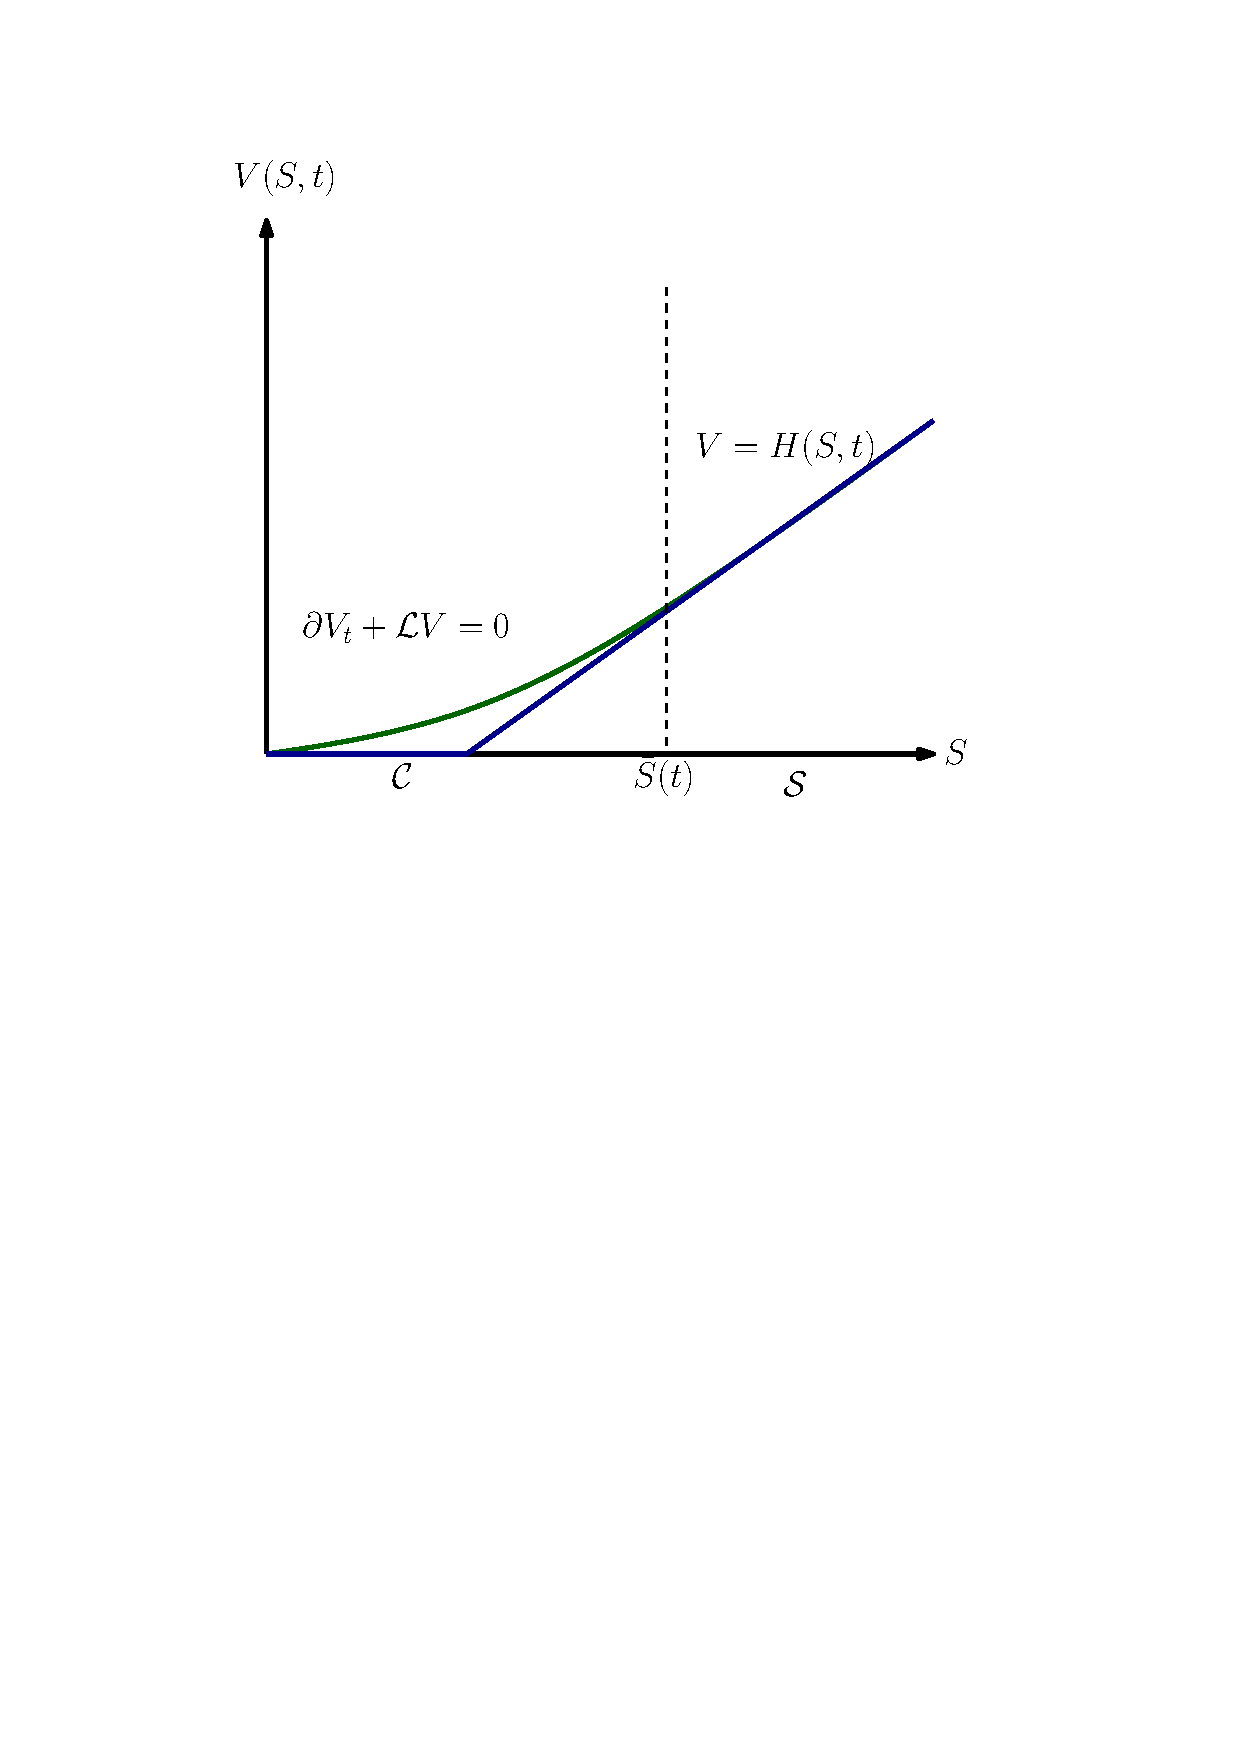
\includegraphics[width=\textwidth]{chapters/chapter2/AmericanCallOptionValue}
    \caption{Call option}
    \label{fig:blackscholes:preliminaries:american_call_value_vs_curve}
  \end{subfigure}
  \hfill
  \begin{subfigure}{0.4\textwidth}
    \centering
    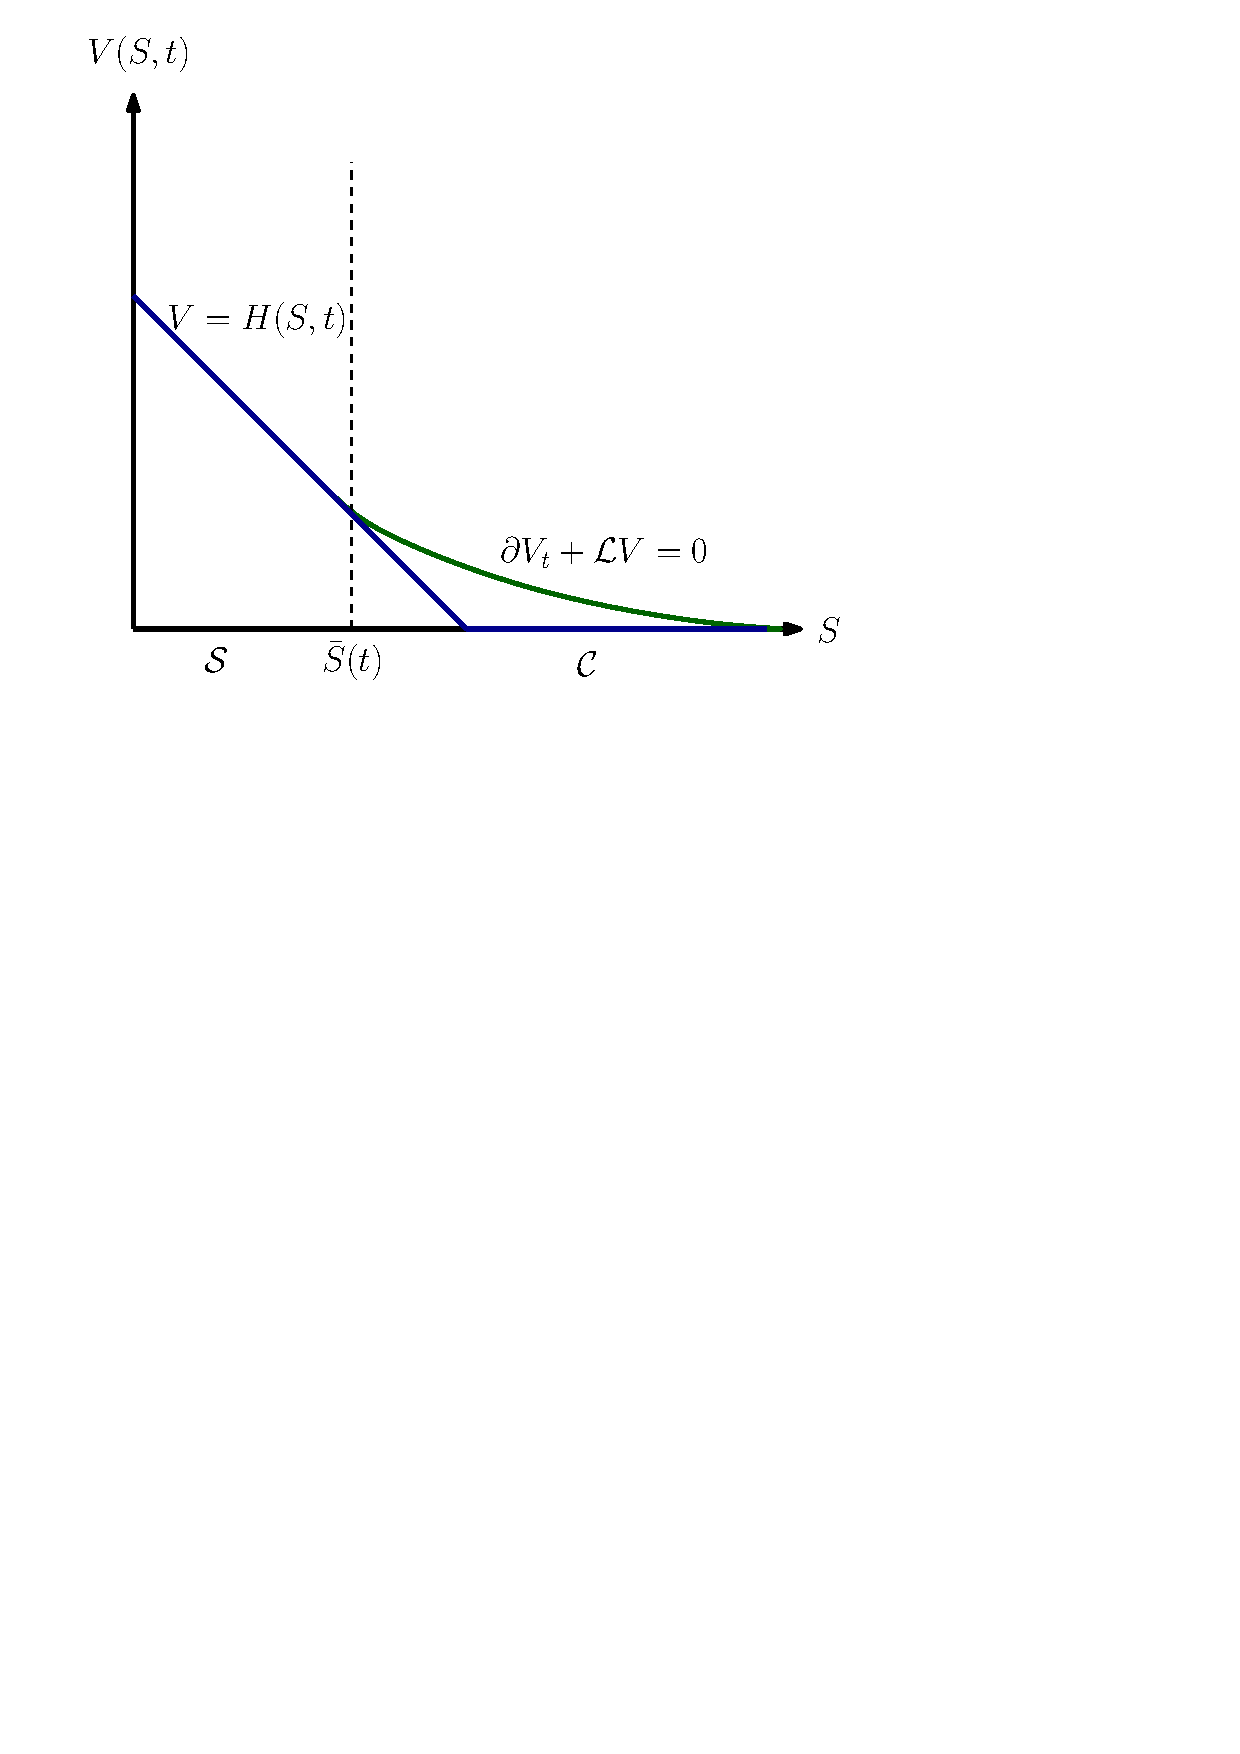
\includegraphics[width=\textwidth]{chapters/chapter2/AmericanPutOptionValue.pdf}
    \caption{Put option}
    \label{fig:blackscholes:preliminaries:american_put_value_vs_curve}
  \end{subfigure}
  \caption{Value $V(S, t)$ of American option value curve. }
  \label{fig:blackscholes:preliminaries:american_option_value_vs_curve}
\end{figure}
and, lastly, that the price dynamics of
American options is governed by the same Black-Scholes PDE as European options in the continuation region. Therefore, Pricing American options reduces to solve \eqref{eq:blackscholes:preliminaries:european_option_pde} with a boundary condition at the optimal exercise price $\bar{S}(t)$.
\begin{align}
  \begin{cases}
    \dfrac{\partial{V}}{\partial{t}} + \dfrac{1}{2}\sigma^{2} S^2 \dfrac{\partial^2{V}}{\partial{S^2}} + (r - \delta)S \dfrac{\partial{V}}{\partial{S}} - rV = 0 & \text{for $(S, t) \in \mathcal{C}$} \\ V(S, t) = H(S, t) &
    \text{for $(S,t)\in \partial\mathcal{C}$}
  \end{cases}
  \label{eq:blackscholes:preliminaries:american_options_pde_free_boundary_problem}
\end{align}
The problem above is also known as the free boundary formulation of the pricing problem because it requires to solve a PDE with a moving boundary. Clearly, the optimal exercise price $\bar{S}(t)$ is within the exercise region \eqref{eq:blackscholes:preliminaries:exercise_region}. Moreover, the boundary condition opposite the moving boundary are
\begin{subequations}
  \begin{align}
    \text{\textbf{Call:}} \quad& V(0,t) = 0, \quad V(\bar{S}(t),t) = \bar{S}(t) - K\\
    \text{\textbf{Put:}} \quad& V(\bar{S},t) = K - \bar{S}(t), \quad \lim_{\infty}V(S, t)=0
    \label{eq:blackscholes:preliminaries:american_options_boundary_conditions}
  \end{align}
\end{subequations}
Additionally, it can be observed in figure \eqref{fig:blackscholes:preliminaries:american_option_value_vs_curve} that $V(S,t)$ touches the payoff $H(S,t)$ tangentially at the optimal exercise price $\bar{S}(t)$ 
\begin{subequations} \label{eq:blackscholes:preliminaries:smooth_passing_condition}
  \begin{align}
    \text{\textbf{Call:}} \qquad &\dfrac{\partial{V}}{\partial{S}}(\bar{S}(t), t) = 1\\
    \text{\textbf{Put:}} \qquad &\dfrac{\partial{V}}{\partial{S}}(\bar{S}(t), t) = -1
  \end{align}
\end{subequations}
This extra condition is called the contact point or smooth pasting condition and later on will serve handy in approximating $\bar{S}(t)$. Finally, the terminal condition of the PDE will be given at $t=T$. At the expiration date of the contract, the holder will either exercise or not the option. Therefore, the value of the option will be equal to the payoff function. Obviously, in that case, the optimal exercise price $S(T)$ will be equal to the strike price $K$. Hence,
\begin{align}
  V(S,T) = H(S, T), \qquad \bar{S}(T) = K
  \label{eq:blackscholes:preliminaries:american_options_terminal_condition}
\end{align}
By grouping \eqref{eq:blackscholes:preliminaries:american_options_pde_free_boundary_problem}, \eqref{eq:blackscholes:preliminaries:smooth_passing_condition}, and \eqref{eq:blackscholes:preliminaries:american_options_terminal_condition} in one equation, a system for the free boundary problem is obtained.
\begin{subequations} \label{eq:blackscholes:preliminaries:american_options_pde_free_boundary_problem_full}
  \begin{align}
    \label{eq:blackscholes:preliminaries:call_american_options_pde_free_boundary_problem_full}
    \text{\textbf{Call}:} \quad &
    \begin{cases}
      \dfrac{\partial{V}}{\partial{t}} + \dfrac{1}{2}\sigma^{2} S^2 \dfrac{\partial^2{V}}{\partial{S}^2} + (r - \delta)S\dfrac{\partial{V}}{\partial{S}} - rV = 0 & \text{for $S \in (0,\bar{S}(t))$ and $t \in [0, T)$} \\ 
      V(S, T) = S - K \\
      \bar{S}(T) = K \\ 
      V(0, t) = 0 \\
      \dfrac{\partial{V}}{\partial{S}}(\bar{S}(t), t) = 1
    \end{cases} \\
    \text{\textbf{Put}:} \quad &
    \begin{cases}
      \dfrac{\partial{V}}{\partial{t}} + \dfrac{1}{2}\sigma^{2} S^2 \dfrac{\partial^2{V}}{\partial{S}^2} + (r - \delta)S\dfrac{\partial{V}}{\partial{S}} - rV = 0 & \text{for $S \in (\bar{S}(t), \infty)$, and $t \in [0, T)$} \\
      V(S, T) = K - S \\
      \bar{S}(T) = K \\ 
      \lim_{S\rightarrow\infty}V(S, t) = 0 \\ 
      \dfrac{\partial{V}}{\partial{S}}(\bar{S}(t), t) = -1
    \end{cases}
  \end{align}
\end{subequations}
\newpage
\subsection{Front-Fixing method}
In the previous section, we presented the pricing  problem for American options problem. By applying the Black-Scholes model, we derived the Black-Scholes PDE that describes the price dynamics in the continuation region $\mathcal{C}$ of call and put options. Also, we introduced the moving boundary condition $\bar{S}(t)$ for the Black-Scholes PDE. The moving boundary condition $\bar{S}(t)$ makes solving the Black-Scholes PDE more involving since the free boundary is an unknown function of time. This type of problems are known as free boundary problems. The front fixing method is a strategy in which a transformation is used to map the  domain from the original problem to a new domain where the moving boundary remains fixed as time changes. In this section, we explore two transformation based on the work of Nielsen et al.\cite{nielsen_2001}, and the work of Company and et al.\cite{company_egorova_jodar_2014}.
\subsubsection{Nielsen transformation} \label{sec:blackscholes:frontfixingmethod:nielsen}
The Nielsen transformation suggests a really simple change of variable in which
the asset price $S$ is divided by the optimal exercise price $\bar{S}$
\begin{equation}
  x = \dfrac{S}{\bar{S}(t)}
  \label{eq:blackscholes:frontfixingmethod:nielsen}
\end{equation}
Clearly, the moving boundary in the original problem will be fixed when $S=\bar{S}(t)$ at $x=1$. Now, we define $v(x,t)$ as the value function of the option but under the front fixing domain given by $x$
\begin{equation}
  v(x, t) := V(S, t)
  \label{eq:blackscholes:frontfixingmethod:nielsen:value_function}
\end{equation}
Moreover, we want to understand how this transformation affects the Black-Scholes PDE, the boundary, terminal and contact point conditions given in equation in \eqref{eq:blackscholes:preliminaries:american_options_pde_free_boundary_problem_full}.

Firstly, we start with the Black-Scholes PDE which is defined at the interval 
$S\in(0, \bar{S}(t))$ for call options or the open interval $S\in(\bar{S}(t), \infty)$ for put options. Under the front fixing domain, the transformed PDE will be defined in the interval $x\in(0, 1)$ for call and $x\in(1, \infty)$ for put options, respectively. Moreover, we apply the chain rule to rewrite the Black-Scholes PDE in terms of $v(x,t)$
\begin{subequations} \label{eq:blackscholes:frontfixingmethod:nielsen:american_options_pde}
  \begin{align}
    \text{\textbf{Call:}} \qquad
    \dfrac{\partial{v}}{\partial{t}} + \dfrac{1}{2}\sigma^{2} x^2 \dfrac{\partial^2{v}}{\partial{x}^2} + \bigg[(r - \delta) - \dfrac{\bar{S}^\prime(t)}{\bar{S}(t)}\bigg]x\dfrac{\partial{v}}{\partial{x}} - rv = 0 \quad & \text{for $x \in [0, 1)$ and $t \in [0, T)$} \\
    \text{\textbf{Put:}} \qquad
    \dfrac{\partial{v}}{\partial{t}} + \dfrac{1}{2}\sigma^{2} x^2 \dfrac{\partial^2{v}}{\partial{x}^2} + \bigg[(r - \delta) - \dfrac{\bar{S}^\prime(t)}{\bar{S}(t)}\bigg]x\dfrac{\partial{v}}{\partial{x}} - rv = 0 \quad & \text{for $x > 1$ and $t \in (0, T]$}
  \end{align}
\end{subequations}
Similarly, we express the boundary conditions in the front fixing domain. We already stated that the Nielsen transformation fixes the moving boundary $\bar{S}$ at $x=1$. Additionally, $x$ goes to infinity as $S$ goes to infinity, and $x=0$ for $S=0$. Therefore, the boundary condition opposite to the optimal exercise price $\bar{S}(t)$ will remain as in the original problem (See figure \ref{fig:blackscholes:preliminaries:american_option_value_vs_curve} and \ref{fig:blackscholes:frontfixingmethod:nielsen_value_vs_curve}). Hence, the call option has left boundary condition $v(0, t) = 0$ at $x=0$ and right boundary condition $v(1, t) = \bar{S}(t) - K$ at $x=1$. Alternatively, 
the put option has left boundary condition $v(1, t) = K - \bar{S}(t)$ at $x=1$ and right boundary condition $v(x, t) = 0$ at a sufficiently large $x$.
\begin{figure}[H]
  \centering
  \begin{subfigure}{0.45\textwidth}
    \centering
    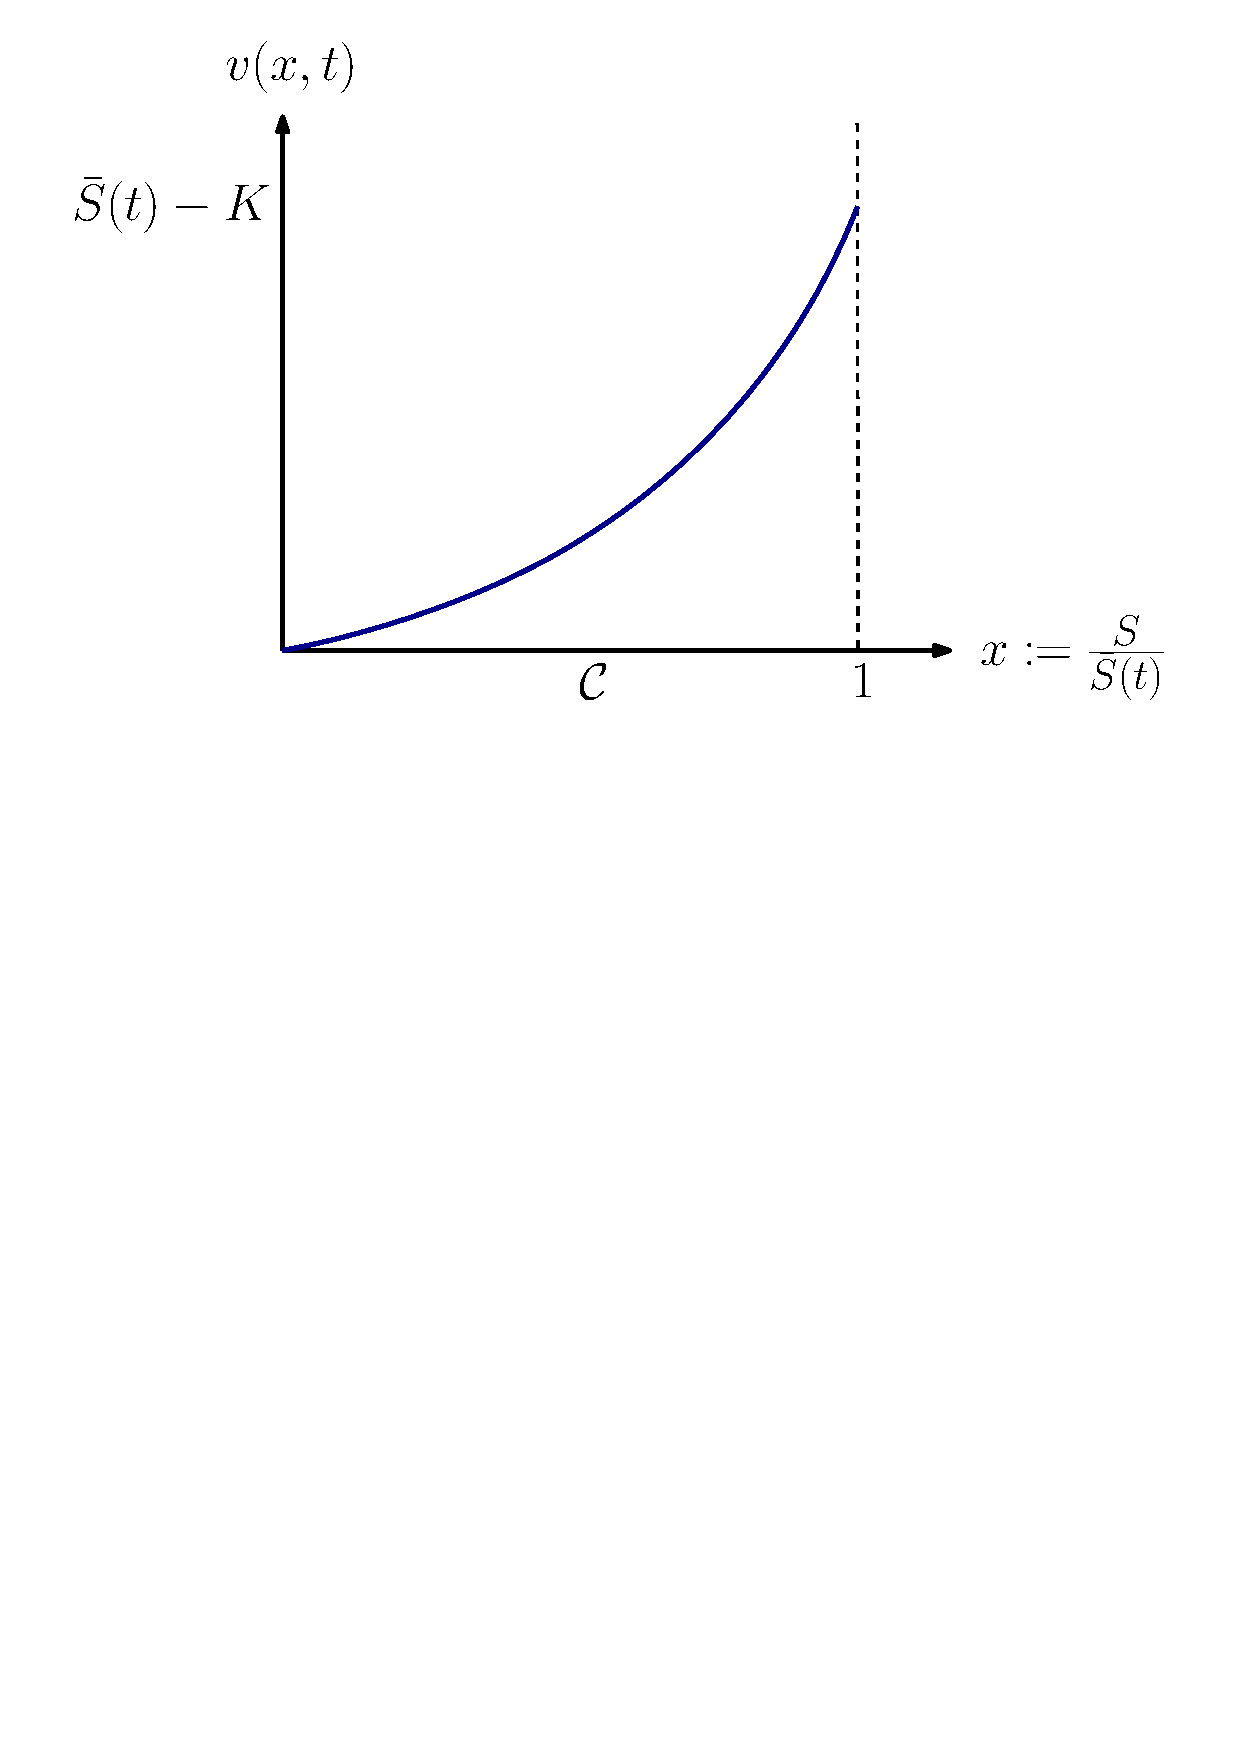
\includegraphics[width=\textwidth]{chapters/chapter2/NielsenCallOption}
    \caption{Call option}
    \label{fig:blackscholes:frontfixingmethod:nielsen_call_value_vs_curve}
  \end{subfigure}
  \begin{subfigure}{0.45\textwidth}
    \centering
    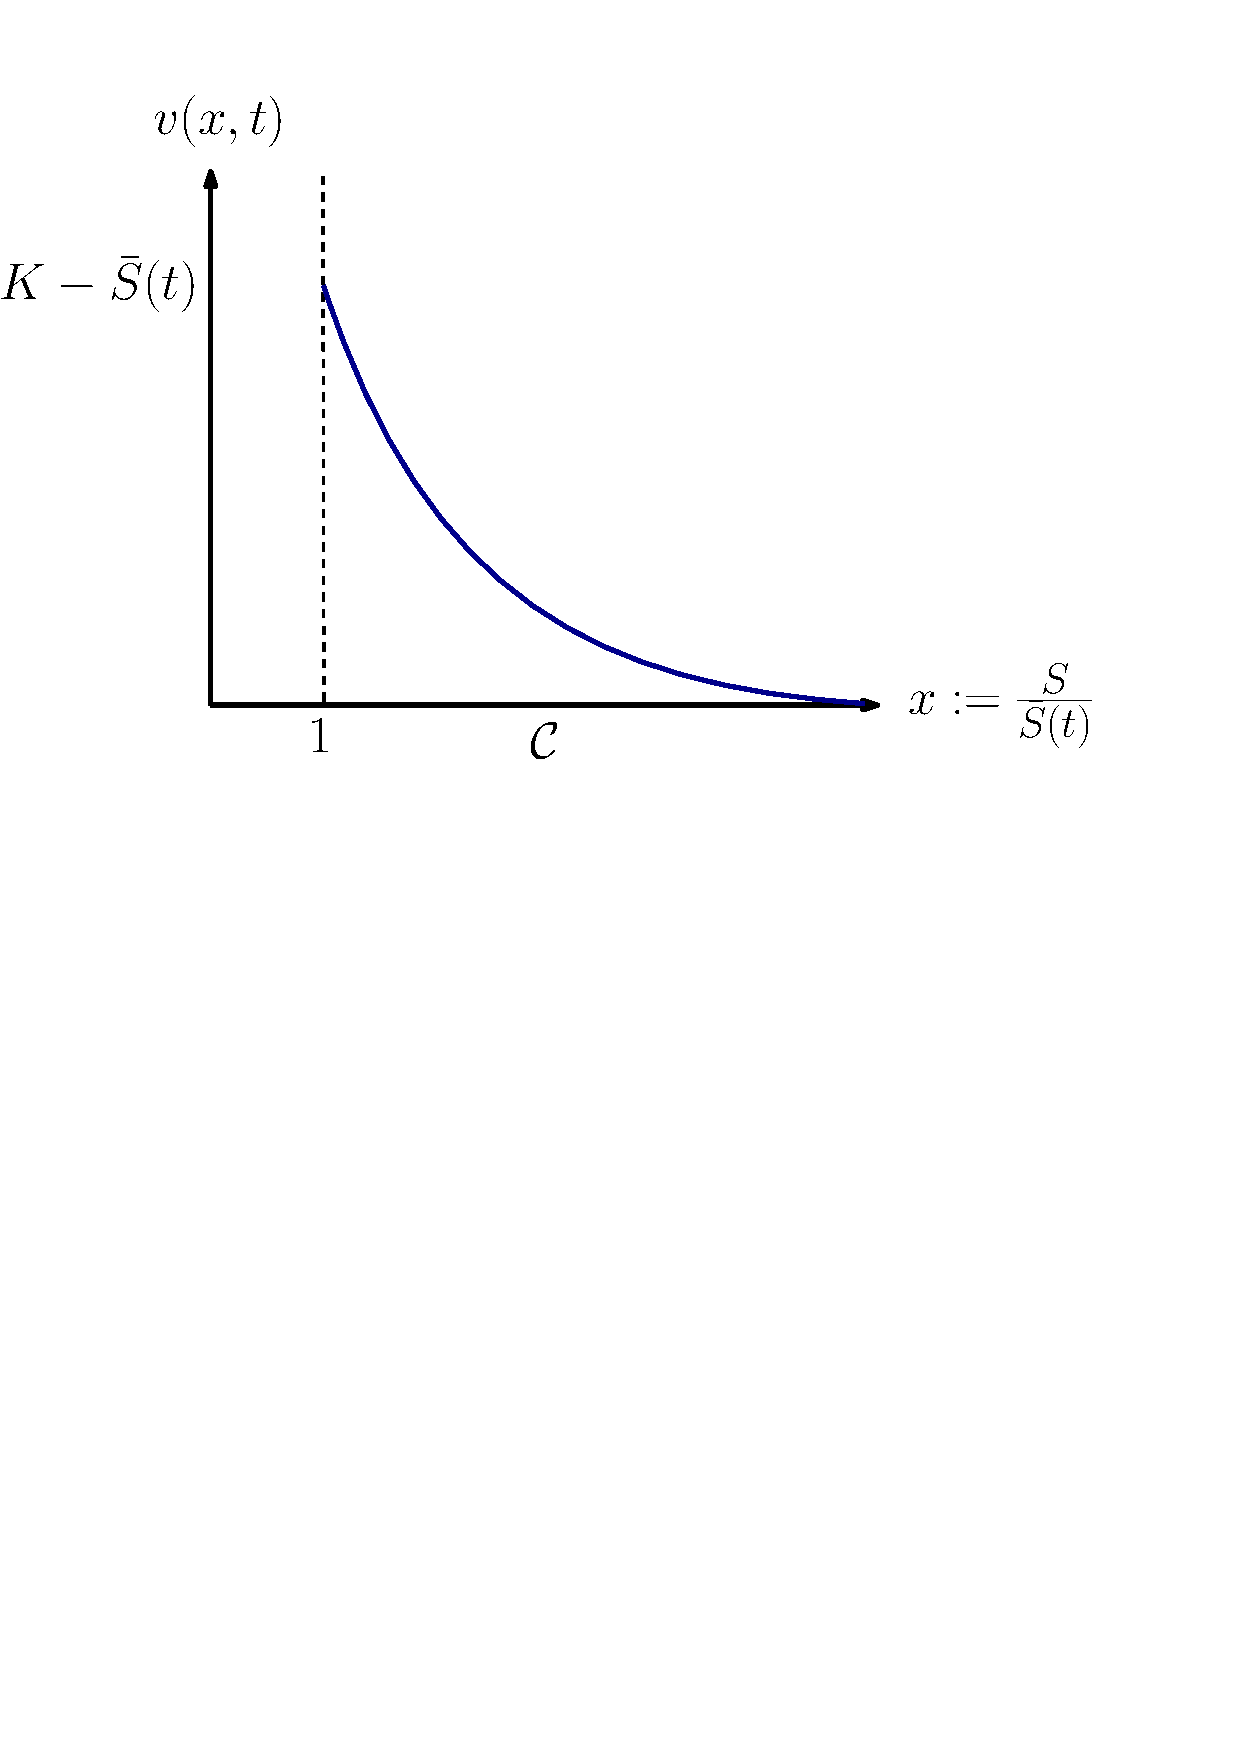
\includegraphics[width=\textwidth]{chapters/chapter2/NielsenPutOption}
    \caption{Put option}
    \label{fig:blackscholes:frontfixingmethod:nielsen_put_value_vs_curve}
  \end{subfigure}
  \caption{Value $v(x,t) := V(S,t)$ in the front fixing domain defined by Nielsen transformation.}
  \label{fig:blackscholes:frontfixingmethod:nielsen_value_vs_curve}
\end{figure}
Likewise, we express the contact point condition in terms of $v(x,t)$. Recall that at the contact point, the slope $V(S,t)$ with respect to $S$ is the same as the slope of the line segment in the payoff function (See figure \ref{fig:blackscholes:preliminaries:american_option_value_vs_curve}). Hence, by the chain rule, the contact point condition of $v(x,t)$ is
\begin{subequations} \label{eq:blackscholes:frontfixingmethod:nielsen:american_options_optimal_price_contact_point_condition}
  \begin{align}
    \text{\textbf{Call:}} \qquad & \dfrac{\partial v}{\partial x}(1, t) = \bar{S}(t) \\
    \text{\textbf{Put:}} \qquad & \dfrac{\partial v}{\partial x}(1, t) = -\bar{S}(t)
  \end{align}
\end{subequations}
Finally, recall that the terminal condition of $\bar{S}(t)$ is given by \eqref{eq:blackscholes:preliminaries:american_options_terminal_condition}. Moreover,
$x>=1$ for call options, and $x<=1$ for put options. Hence, by simple substitution, we can rewrite the terminal conditions of $v(x, t)$ as
\begin{subequations} \label{eq:blackscholes:frontfixingmethod:nielsen:american_options_terminal_condition}
  \begin{align}
    \text{\textbf{Call:}} \qquad & v(x, T) = \max(x\bar{S}(T) - K) = K \max(x - 1, 0) = 0 \\
    \text{\textbf{Put:}} \qquad & v(x, T) = \max(K - x\bar{S}(T)) = K \max(1 - x, 0) = 0
  \end{align}
\end{subequations}
In summary, by groping equations
\eqref{eq:blackscholes:frontfixingmethod:nielsen:american_options_pde},
\eqref{eq:blackscholes:frontfixingmethod:nielsen:american_options_terminal_condition}, and
\eqref{eq:blackscholes:frontfixingmethod:nielsen:american_options_optimal_price_contact_point_condition},
we obtain the systems
{
\allowdisplaybreaks  
\begin{subequations} \label{eq:blackscholes:frontfixingmethod:nielsen:american_options_bs_pde}
  \begin{align}
    \text{\textbf{Call:}} \quad &
    \begin{cases}
      \dfrac{\partial{v}}{\partial{t}} + \dfrac{1}{2}\sigma^{2} x^2 \dfrac{\partial^2{v}}{\partial{x}^2} + \bigg[(r - \delta) -
      \dfrac{\bar{S}^\prime(t)}{\bar{S}(t)}\bigg]x\dfrac{\partial{v}}{\partial{x}} - rv = 0 & \text{for $x \in (0, 1)$ and $t \in [0, T)$} \\ 
      v(x, T) = 0 & \text{for $x\in[0, 1]$}  \\
      \bar{S}(T) = K \\ 
      v(0, t) = 0 & \text{for $t\in[0, T)$}\\ 
      v(1, t) = \bar{S}(t) - K & \text{for $t\in[0, T)$}\\ 
      \dfrac{\partial{v}}{\partial{x}}(1, t) = \bar{S}(t) & \text{for $t\in[0, T)$}
    \end{cases}\\
    \text{\textbf{Put:}} \quad &
    \begin{cases}
      \dfrac{\partial{v}}{\partial{t}} + \dfrac{1}{2}\sigma^{2} x^2 \dfrac{\partial^2{v}}{\partial{x}^2} + \bigg[(r - \delta) -
      \dfrac{\bar{S}^\prime(t)}{\bar{S}(t)}\bigg]x\dfrac{\partial{v}}{\partial{x}} - rv = 0 & \text{for $x > 1$ and $t \in [0, T)$} \\ 
      v(x, T) = 0 & \text{for $x \ge 1$} \\
      \bar{S}(T) = K \\ 
      v(1, t) = K - \bar{S}(t) & \text{for $t\in[0, T)$} \\
      \lim_{x\rightarrow\infty}v(x, t) = 0 & \text{for $t\in[0, T)$} \\
      \dfrac{\partial{v}}{\partial{x}}(1, t) = -\bar{S}(t) & \text{for $t\in[0, T)$}
    \end{cases}
  \end{align}
\end{subequations}
}
\subsubsection{Company transformation}
The Company transformation proposes set of change of variables for the asset price $S$, the time $t$, the value function $V(S,t)$ and the moving boundary
\begin{equation}
  x := \log \dfrac{S}{\bar{S}_f(t)}, \quad \tau := T - t, \quad v(x, \tau) := \dfrac{V(S, t)}{K}, \quad \bar{S}_f(\tau) := \dfrac{\bar{S}(t)}{K} 
\end{equation}
Let us break down the transformations. Firstly, the transformation proposed are written backward in time. Therefore, $\tau = 0$ refers to the expiration date of the options $t=T$. Secondly, both the value function and the optimal exercise price is scaled by the strike price. Finally, the new moving boundary is fixed at $S=\bar{S}_f(t)$ or $x=0$.

Similarly, as we did for the Nielsen method, we rewrite the Black-Scholes PDE in terms of $v(x, \tau)$. Note that as $x$ goes to infinity $S$ goes to infinity. Conversely, as $x$ goes to negative infinity $S$ goes to zero. Moreover, $S=\bar{S}(t)$ at $x=0$. Using the previous information, we deduce  that the Black-Scholes PDE is defined in the intervals $x\in(-\infty, 0)$ for call options and $x\in(0, \infty)$ for put options. Therefore, we have
{
\allowdisplaybreaks 
\begin{subequations}
  \begin{align}
      \text{\textbf{Call:}} \quad \dfrac{\partial v}{\partial \tau} - \dfrac{1}{2}\sigma^2\dfrac{\partial^2 v}{\partial x^2} - \bigg((r-\delta) + \dfrac{\sigma^2}{2} - \dfrac{\bar{S}'(\tau)}{\bar{S}(\tau)} \bigg)\dfrac{\partial v}{\partial x} + rv = 0 \quad \text{for $x < 0$ and $\tau \in (0, T]$} \\
      \text{\textbf{Put:}} \quad \dfrac{\partial v}{\partial \tau} - \dfrac{1}{2}\sigma^2\dfrac{\partial^2 v}{\partial x^2} - \bigg((r-\delta) - \dfrac{\sigma^2}{2} - \dfrac{\bar{S}'(\tau)}{\bar{S}(\tau)} \bigg)\dfrac{\partial v}{\partial x} + rv = 0 \quad \text{for $x > 0$ and $\tau \in (0, T]$}
  \end{align}
\end{subequations}
}
Note that the term on the new PDE that correspond to the terms in the linear parabolic operator $\mathcal{L}_\text{BS}(V)$ defined in \eqref{eq:blackscholes:preliminaries:linear_parabolic_operator} are negative because the Black-Scholes PDE was written backward in time.

The boundary conditions for the call option in the original domain are
$V(0,t)$ at $S=0$ and $V(\bar{S}, t) = \bar{S} - K$  at $S=\bar{S}(t)$, and when transforming those boundary conditions to the front fixing domain, they become $v(x, \tau) = 0$ for a sufficiently negative $x$ and $v(0, \tau) := \bar{S}_f(\tau) - 1 = V(\bar{S}, t) / K$ at $x=0$. Similarly, the boundary conditions for the put option in the original domain are $V(\bar{S}(t), t) = K - \bar{S}$ at $S=\bar{S}(t)$ and $V(S, t) = 0$ for a sufficiently large $S$, and under the front fixing domain, they become $v(0, \tau) = 1 - \bar{S}_f(\tau) = V(\bar{S}, t) / K$ at $x=0$ and $v(x, \tau) = 0$ for a sufficiently large $x$. Similarly, to as we did for the Nielsen transformation, we also rewrite the contact point condition
\begin{subequations}
  \begin{align}
    \text{\textbf{Call:}} \qquad & \dfrac{\partial v}{\partial x}(0, \tau) =  \bar{S}_f(\tau)\\
    \text{\textbf{Put:}} \qquad & \dfrac{\partial v}{\partial x}(0, \tau) = -\bar{S}_f(\tau)
  \end{align}
\end{subequations}
\begin{figure}[H]
  \centering
  \begin{subfigure}{0.265\textheight}
    \centering
    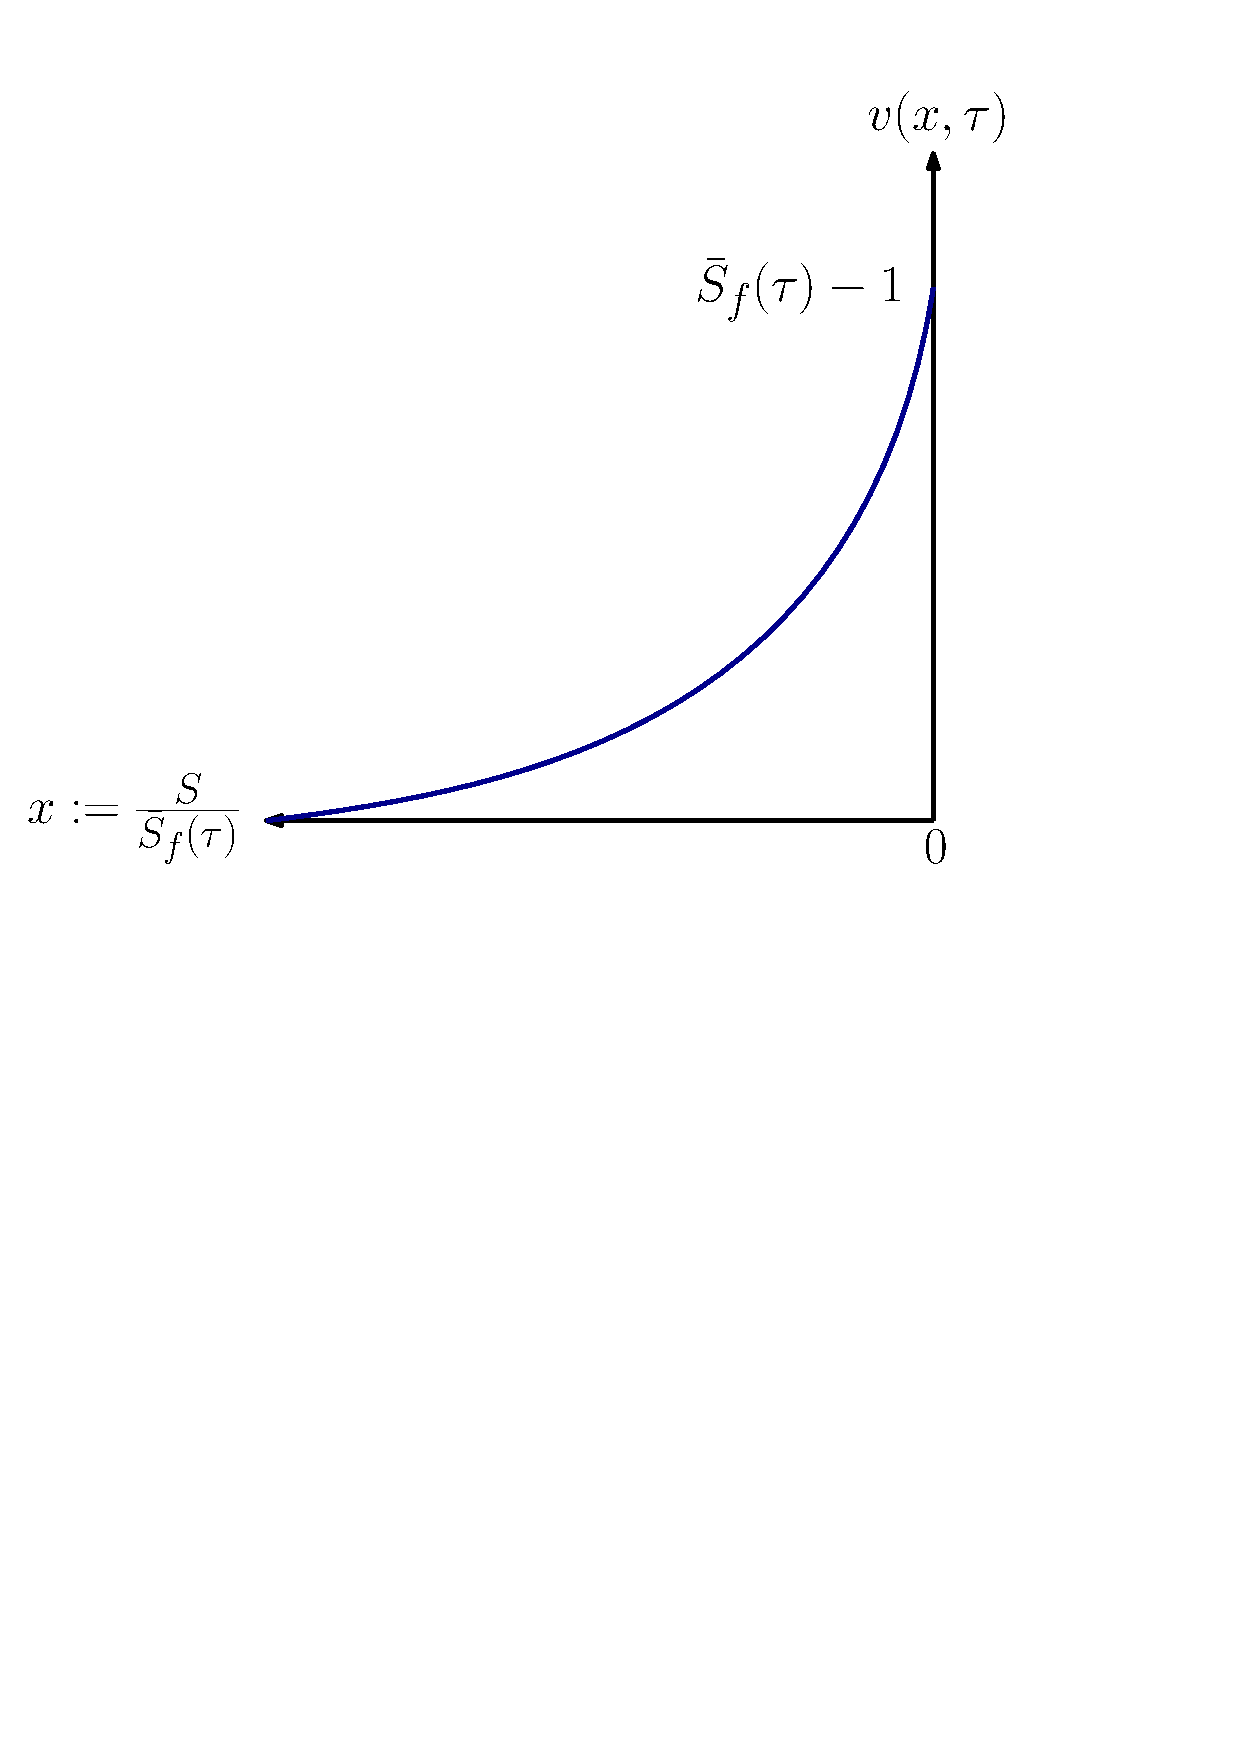
\includegraphics[width=\textwidth]{chapters/chapter2/CompanyCallOption.pdf}
    \caption{Call option}
    \label{fig:blackscholes:frontfixingmethod:company_call_value_vs_curve}
  \end{subfigure}
  \begin{subfigure}{0.305\textheight}
    \centering
    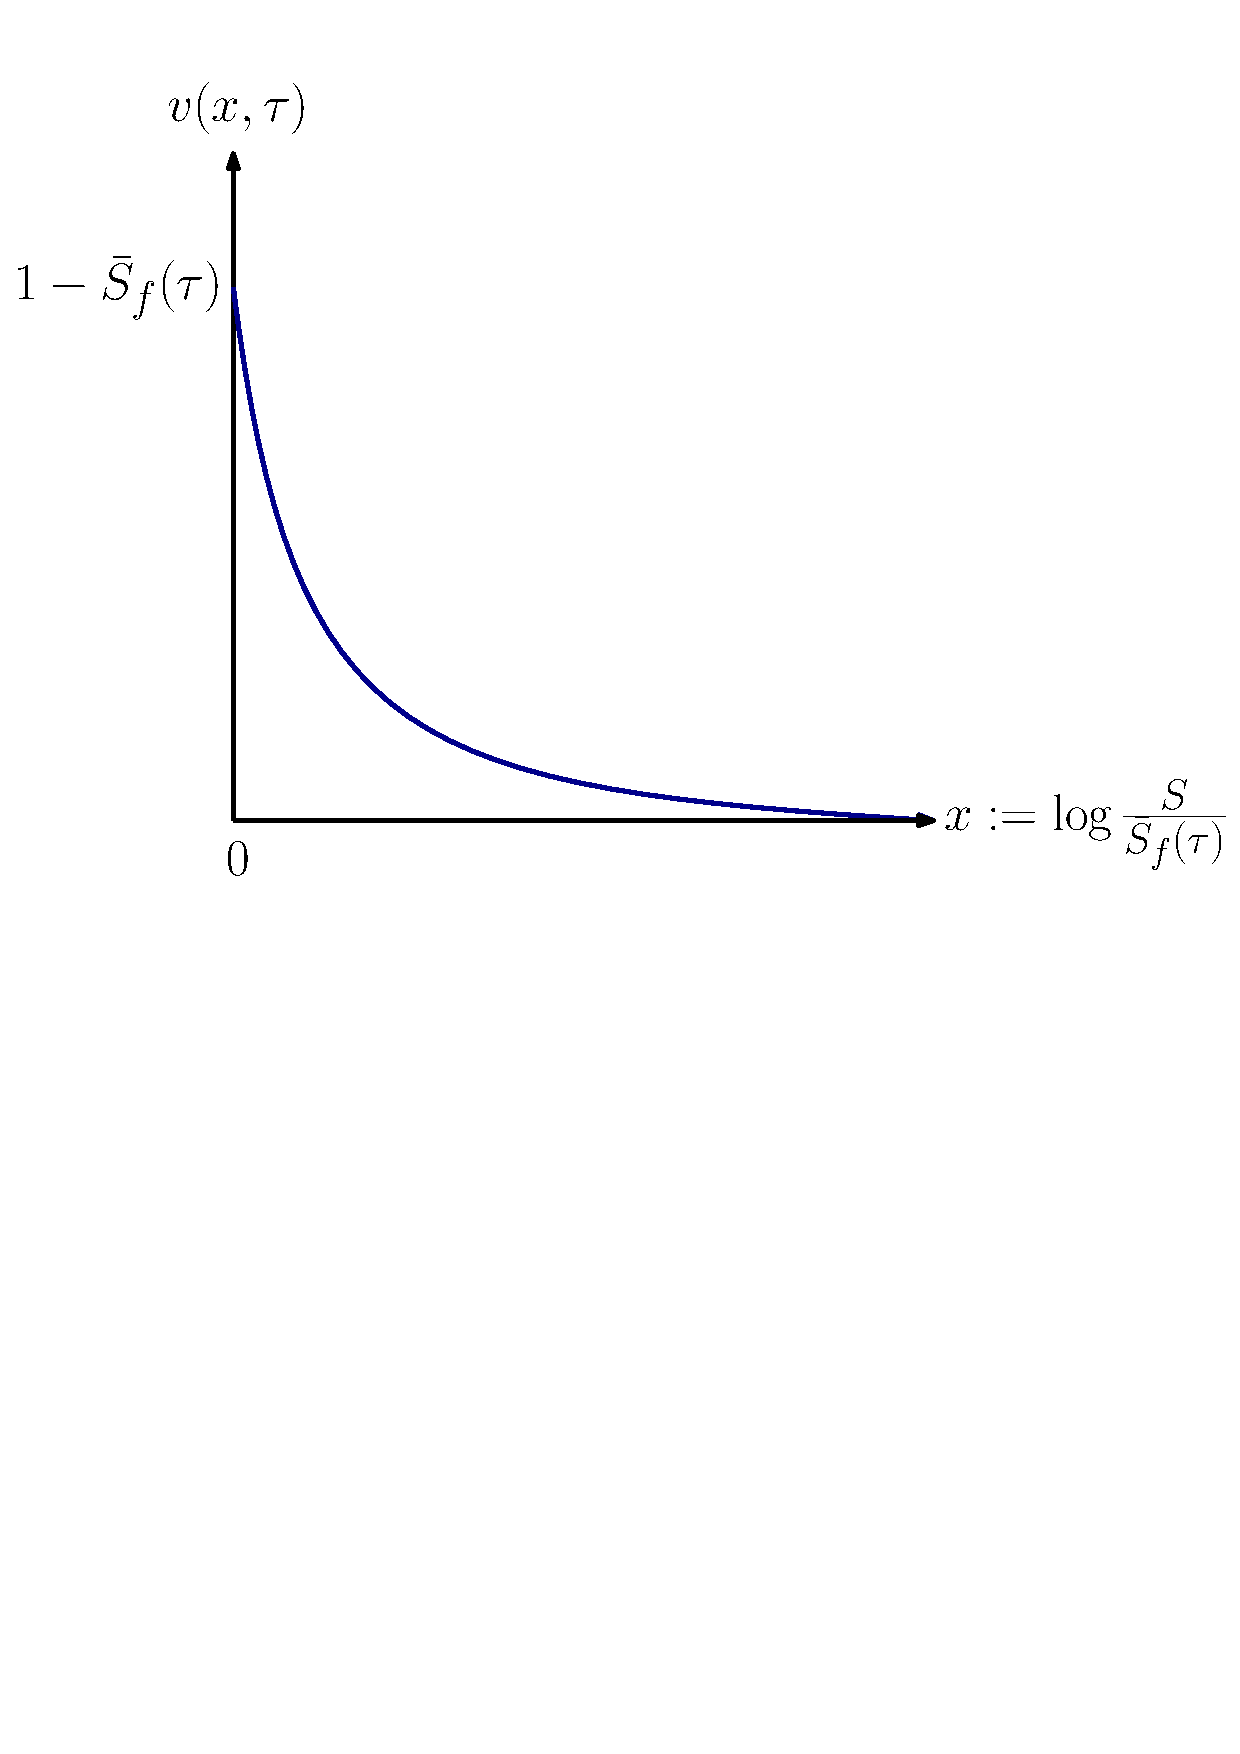
\includegraphics[width=\textwidth]{chapters/chapter2/CompanyPutOption.pdf}
    \caption{Put option}
    \label{fig:blackscholes:frontfixingmethod:company_put_value_vs_curve}
  \end{subfigure}
  \caption{Value $v(x,t) := V(S,t) / K$ in the front fixing domain defined by Company transformation.}
  \label{fig:blackscholes:frontfixingmethod:company_value_vs_curve}
\end{figure}
Since the transformed PDE is backward in time, we have to come up with initial conditions for $\bar{S}_f(\tau)$ and $v(x, \tau)$. For $\bar{S}_f(\tau)$, the initial condition is given by
\begin{equation}
  \bar{S}_f(0) = \dfrac{\bar{S}(T)}{K} = 1
\end{equation}
Moreover, for call options, the initial condition is given by $v(x, 0) = V(S, T) / K = \max\big(\bar{S}_f(0)e^{x} - 1, 0\big) = \max\big(e^{x} - 1, 0\big) = 0$ since $x$ is always negative. Similarly, for put options, the initial condition is given by $v(x, 0) = V(S, T) / K = \max\big(1 - \bar{S}_f(0)e^x, 0\big) = \max\big(1 - e^x, 0\big) = 0$ since $x$ is always positive. Hence,
\begin{subequations} \label{eq:blackscholes:frontfixingmethod:logtransform:american_options_terminal_condition}
  \begin{align}
    \text{\textbf{Call:}} \qquad & v(x, 0) = 0 \\
    \text{\textbf{Put:}} \qquad & v(x, 0) = 0
  \end{align}
\end{subequations}
Finally, grouping the equations together, we have the system
\begin{subequations} \label{eq:blackscholes:frontfixingmethod:logtransform:american_options_bs_pde}
  \begin{align}
    \text{\textbf{Call:}} \quad &
    \begin{cases}
      \dfrac{\partial v}{\partial \tau} - \dfrac{1}{2}\sigma^2\dfrac{\partial^2 v}{\partial x^2} - \bigg((r-\delta) + \dfrac{\sigma^2}{2} - \dfrac{\bar{S}'(\tau)}{\bar{S}(\tau)} \bigg)\dfrac{\partial v}{\partial x} + rv = 0 & \text{for $x < 0$ and $\tau \in (0, T]$}  \\ 
      v(x, 0) = 0 & \text{for $x < 0$} \\ 
      \bar{S}_f(0) = 1  \\ 
      \lim_{x\rightarrow-\infty}{v(x, \tau)} = 0 & \text{for $\tau \in (0, T]$}  \\ 
      \dfrac{\partial{v}}{\partial{x}}(0, \tau) = \bar{S}_f(\tau) & \text{for $\tau \in (0, T]$} 
    \end{cases} \\
    \text{\textbf{Put:}} \quad &
    \begin{cases}
      \dfrac{\partial v}{\partial \tau} - \dfrac{1}{2}\sigma^2\dfrac{\partial^2 v}{\partial x^2} - \bigg((r-\delta) - \dfrac{\sigma^2}{2} - \dfrac{\bar{S}'(\tau)}{\bar{S}(\tau)} \bigg)\dfrac{\partial v}{\partial x} + rv = 0 & \text{for $x > 0$ and $\tau \in (0, T]$} \\ 
      v(x, 0) = 0 & \text{for $x > 0$}\\
      \bar{S}_f(0) = 1 \\ 
      \lim_{x\rightarrow\infty} v(x, \tau) = 0 & \text{for $\tau \in (0, T]$} \\ 
      \dfrac{\partial{v}}{\partial{x}}(0, \tau) = -\bar{S}_f(\tau) & \text{for $\tau \in (0, T]$}
    \end{cases}
  \end{align}
\end{subequations}